%==============================================================================
%  Problem 1.C -- cruise control free-body diagram.
%
%  Redrawn from 1_C_schematic.drawio so the labels are text: edit a name here
%  and rebuild with `make`, which exports this file to
%  figures/1_C_free_body.pdf. The standalone class crops the page to the
%  drawing, so \answerfigure scales it with no stray margin.
%
%  Upper panel: the car in side view, travelling right with velocity v and
%  acceleration \dot{v}. Lower panel: the same car as a free body of mass m,
%  driven right by the engine force u and retarded by the friction force bv.
%==============================================================================
\documentclass[border=4pt]{standalone}
\usepackage{amsmath}
\usepackage{tikz}
\usetikzlibrary{patterns,arrows.meta}

\begin{document}
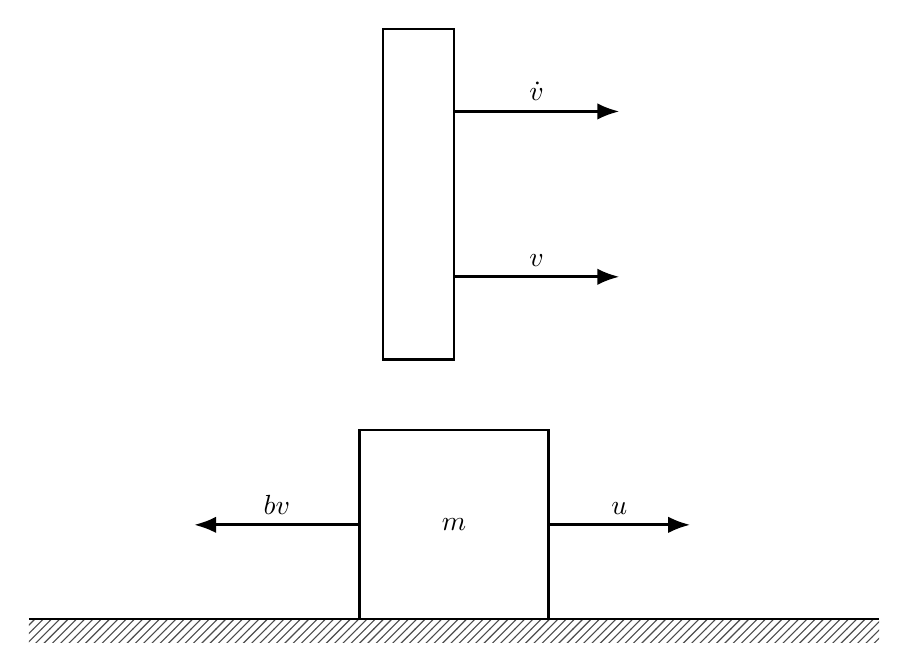
\begin{tikzpicture}[
  line width=0.8pt,
  % Hatching for anything rigidly fixed to ground: walls, ceilings, roads.
  hatch/.style={pattern=north east lines,pattern color=black!70,draw=none},
  body/.style={draw,fill=white},
  force/.style={-{Latex[length=2.8mm]},line width=1pt},
  lbl/.style={font=\normalsize},
]

%--- geometry ----------------------------------------------------------------
\def\roadL{0}          % left end of the road
\def\roadR{10.8}       % right end of the road
\def\roadT{1.8}        % road surface, where the mass sits
\def\hatchw{0.3}       % thickness of the hatched band

\def\massL{4.2}        % left face of the mass
\def\massR{6.6}        % right face of the mass
\def\massT{4.2}        % top of the mass
\def\forcey{3.0}       % centre line, where the forces act
\def\bvtip{2.1}        % tip of the friction arrow
\def\utip{8.4}         % tip of the engine-force arrow

\def\carL{4.5}         % left face of the car
\def\carR{5.4}         % right face of the car
\def\carB{5.1}         % bottom of the car
\def\carT{9.3}         % top of the car
\def\accy{8.25}        % height of the acceleration arrow
\def\vely{6.15}        % height of the velocity arrow
\def\cartip{7.5}       % tip of both motion arrows

%--- upper panel: the car in side view ---------------------------------------
\draw[body] (\carL,\carB) rectangle (\carR,\carT);

\draw[force] (\carR,\accy) -- (\cartip,\accy)
  node[lbl,midway,above] {$\dot{v}$};
\draw[force] (\carR,\vely) -- (\cartip,\vely)
  node[lbl,midway,above] {$v$};

%--- lower panel: the free body ----------------------------------------------
% The road: a hatched band with a solid surface line on top.
\fill[hatch] (\roadL,\roadT-\hatchw) rectangle (\roadR,\roadT);
\draw (\roadL,\roadT) -- (\roadR,\roadT);

\draw[body] (\massL,\roadT) rectangle (\massR,\massT);
\node[lbl] at ({(\massL+\massR)/2},{(\roadT+\massT)/2}) {$m$};

% Friction opposes the motion, so it points left; the engine force points right.
\draw[force] (\massL,\forcey) -- (\bvtip,\forcey)
  node[lbl,midway,above] {$bv$};
\draw[force] (\massR,\forcey) -- (\utip,\forcey)
  node[lbl,midway,above] {$u$};

\end{tikzpicture}
\end{document}
